\chapter{Experiments}
\label{chap:experiments}

%TODO add wgan experiments
\section{Supervised Baseline}
To the best of the author's knowledge, the closest work using a \ac{vae} is a cross-modal training approach in 3D hand pose estimation \cite{crossmodal}. As there is no similar approach in \ac{hpe} using a \ac{vae}, a supervised model using just a \ac{vae} and 3D ground truth pose data is implemented. This is to verify the feasibility of a \ac{vae} and find a set of hyperparameters that worked well for the H3.6M dataset under the supervised setting. This served as a baseline over which an unsupervised \ac{gan} was built upon. Hyperparameters such as the number of neurons in the layers, the number of residual blocks $n$, dimensions of the latent space, etc are taking as reference.

\section{Unsupervised GAN}
Building upon the supervised \ac{vae}, the proposed architecture is built. The following choice is kept standard for most of the experiments and could be used to reproduce the results. All the layers are made of 1024 neurons. The encoder and the decoder are made of 1 residual block each ($n = 1$) while the discriminator is made of 2. This is to keep the capacity of the generator and the discriminator similar. Various forms of scaling the 2D poses are experimented with to make the cycle of lifting and projection smooth. The scaling mentioned in the preprocessing section where the distance between the root joint and head worked the best. %TODO is this need? is it enough? 

The results presented in the following sections are after training the networks for $\sim$400 epochs (~5.5 hours) on approximately 300,000 2D poses with a batch size of 2560 on an Nvidia Titan X. The input poses are flipped with a probability of 0.5. The model takes 16 joints as the output where the root is added at the origin for validation. The proposed architecture consists of 1024 hidden units per linear layer and 51 latent dimensions. Both the \ac{vae} and the discriminator are trained using Adam optimizer with default hyperparameters and with a learning rate of 2e-4. The gradient norms of the discriminator are clipped to 1 when training the discriminator. While training the generator the gradient norms are clipped to 2 for all the models while the gradient values are clipped to 1000.

One of the challenging parts is finding the optimal weights for each of the terms in the triplet loss. The loss coefficients $\lambda_{recon}$, $\lambda_{\acs{kld}}$, $\lambda_{disc.}$ are set to 1, 0.001, 0.001 respectively. The higher weight is motivated by 2 reasons. $\lambda_{recon}$ refers to the constrained optimization and irrespective of how realistic it is, projection loss is desired to be consistently low to get better \ac{mpjpe}. That leads to the other reason that the quantitative results are given higher importance.
%TODO add loss standardization values to kld

The values of $\lambda{\acs{kld}}$ and $\lambda{disc.}$ can be tuned according to the task at hand based on how well the poses are to be clustered or how important it is to reject poses that are not realistic. The $\beta$ value for the \ac{vae} is cycled from 0 to $\lambda_{\acs{kld}}$ every 40 epochs. While keeping it constant at $\lambda_{\acs{kld}}$ for 10 epochs with a 10 epoch warmup at the beginning of the training.

\section{Quantitative Results}

The results obtained by the networks with the above configuration in addition to the choices mentioned in \ref{chap:method} are summarized in Table \ref{table:result_zv}. The summaries of the models are provided in appendix \ref{chap:summaries} to help reproduction.

\begin{table}[htb!]
    \centering
    \begin{tabularx}{\linewidth}{XXX}%{llcc}
        \toprule
        Supervision  & Algorithm                               & Error (mm) \\
        \midrule \midrule
        Full         & Martinez \etal \cite{MartinezHRL17}     & 37.1       \\
                     & Chen \etal \cite{multiplehypo} (SH, MH) & 42.6       \\
        \midrule
        Weak         & Wandt \etal \cite{repnet}               & 38.2       \\
                     & Drover \etal \cite{can3dpose}           & 38.2       \\
                     & Chen \etal \cite{weaklymultiple} (SH)   & 48.7       \\
                     & Chen \etal \cite{weaklymultiple} (BH)   & 31.6       \\
        \midrule
        Unsupervised & Ching \etal \cite{amazon1}              & 58         \\
                     & Ching \etal \cite{amazon1} (AD) (TD)    & 51         \\
                     & \textbf{Ours}                           & 52.4       \\
                     & \textbf{Ours} (BH)                        & 50         \\
        \bottomrule
    \end{tabularx}
    \caption{}
    \label{table:result_zv}
    \vspace{-3ex}
\end{table}

\textbf{SH} refers to the results using 2D Stacked Hourglass detections as input. These detections are noisy and directly affects the predictions of the model. And \textbf{DA} refers to using Domain Adaptation network to include additional datasets and \textbf{TD} denotes the use of temporal data. It is important to note that the proposed unsupervised method and the one presented in \cite{amazon1} are the only methods that do not predict the scale of the 3D pose due to the processing technique.


\begin{table}[h]
    \centering
    \footnotesize
    % \hspace{-3mm}
    % \tabcolsep=0.1mm
    \begin{tabularx}{\textwidth}{XXXXXXXX}
        \toprule
        R\_Hip & R\_Knee & R\_Ankle    & L\_Hip   & L\_Knee  & L\_Ankle    & Torso    & Neck \\
        \hline
        58.01  & 61.42   & 81.97       & 52.45    & 60.13    & 92.82       & 44.78    & 25.43 \\
        &&&&&&&\\
        Nose   & Head    & L\_Shoulder & L\_Elbow & L\_Wrist & R\_Shoulder & R\_Elbow & R\_Wrist\\
        \hline
        33.39  & 46.29   & 30.48       & 55.72    & 80.84    & 33.53       & 59.23    & 80.05\\
        \bottomrule
    \end{tabularx}
    \caption{Average per joint position error (in mm) for each \textbf{joint} under Protocol $\#2$ using 2D ground truth.}
    \label{table:pjpe}
\end{table}

\begin{table}[h]
    \centering
    \footnotesize
    % \hspace{-3mm}
    % \tabcolsep=0.1mm
    \begin{tabularx}{\textwidth}{XXXXXXXX}
        \toprule
        Directions & Discussion& Eating& Greeting& Phoning& Photo& Posing& Purchases \\
        \hline
        44.37  & 45.14   & 56.64       & 48.15    & 56.47    & 45.06       & 47.33    & 71.30  \\
        &&&&&&&\\
        Sitting& SittingDown& Smoking& Waiting& WalkDog& Walking& WalkTogether& \\
        \hline
        72.08  & 55.01   & 52.47       & 47.37    & 47.51    & 49.53       & 44.61    &  \\
        \bottomrule
    \end{tabularx}
    \caption{Average MPJPE (in mm) for each \textbf{action} under Protocol $\#2$ using 2D ground truth.}
    \label{table:pjpe_a}
\end{table}

The best hypothesis, \textbf{BH} has improved the results by ~2.7 mm which is considerable in comparison to the equivalent gain in \cite{amazon1} using domain adaptation network with more data and temporal information. Since there is no technique to pick the best hypothesis without having access to the ground truth, the results referred to, are the ones obtained using \textbf{ZV} unless specified otherwise. 

\begin{figure}[h]
    \centering
    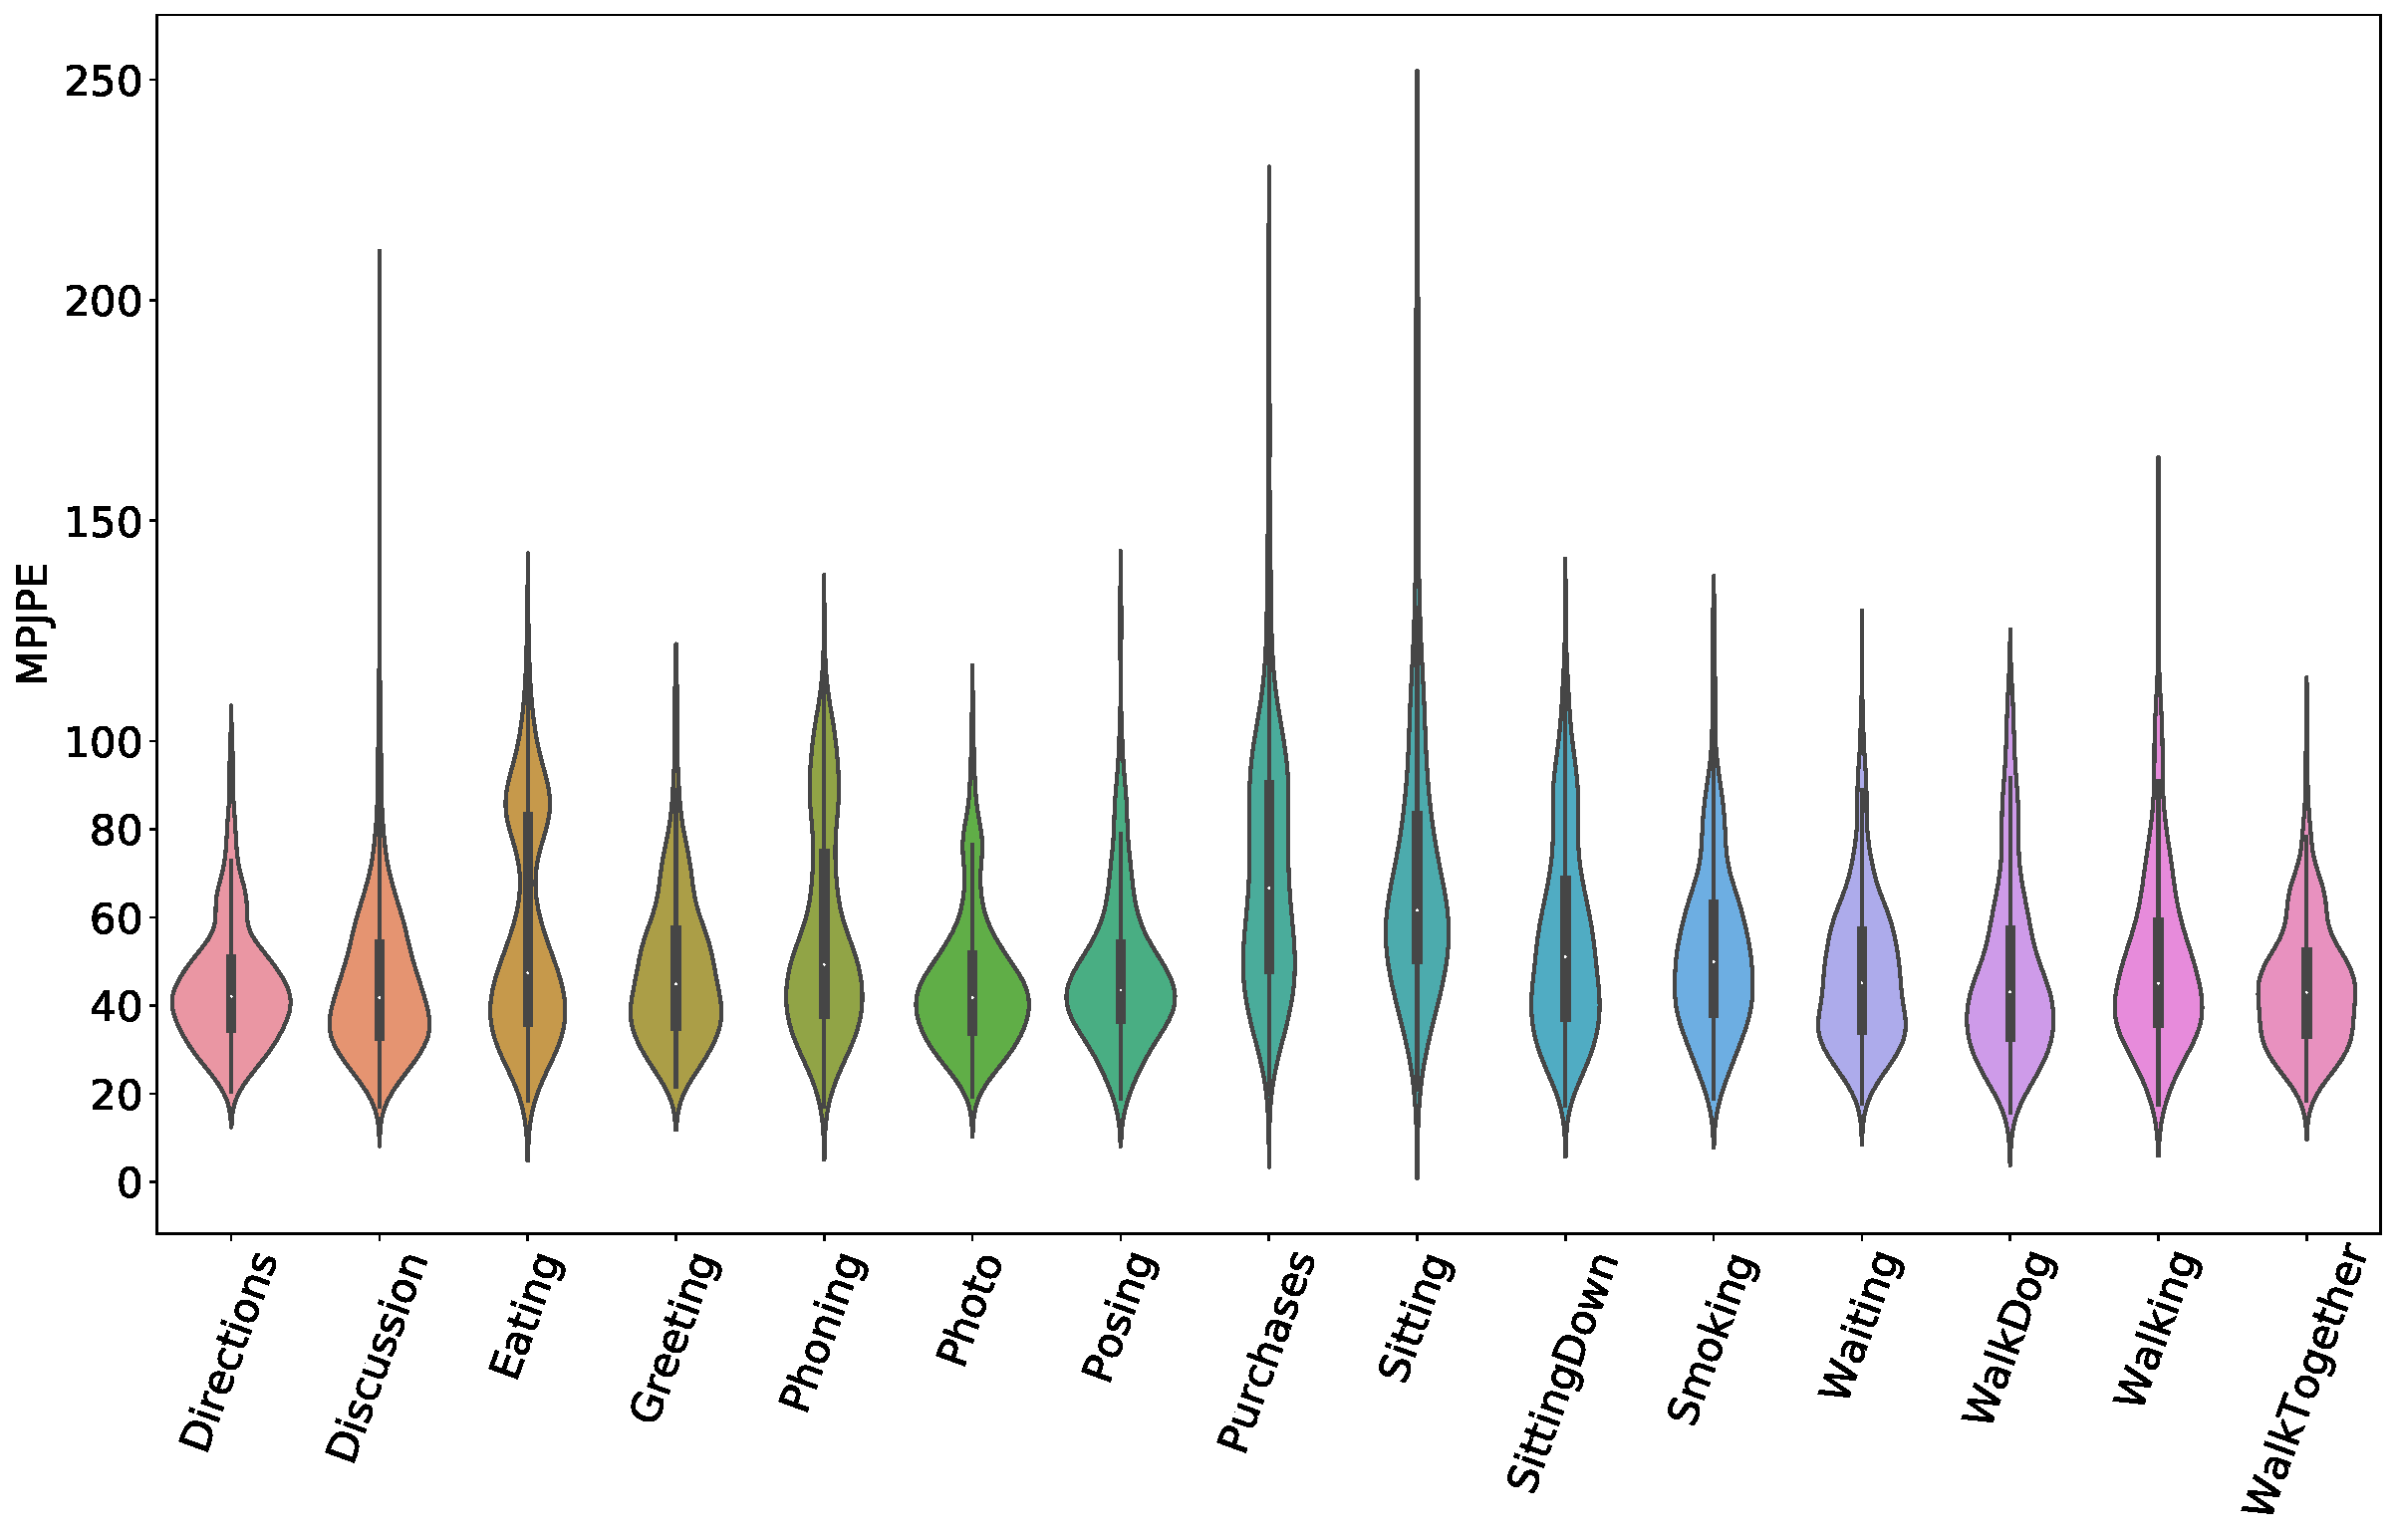
\includegraphics[width=\textwidth]{figures/results/violin_pjpe.pdf}
    \caption{Visualization of the MPJPE error distribution under Protocol $\#2$ for each action.}
    \label{fig:mpjpe_trends}
\end{figure}

The average \ac{mpjpe} errors for each action is presented in Table \ref{table:pjpe_a}, and Fig \ref{fig:mpjpe_trends} illustrates the distribution of these errors. The \ac{mpjpe} error per joint increases as we move from inner to outer joints. This can be observed in Table \ref{table:pjpe} which shows the average per joint position error. The error for the Pelvis joint is not mentioned as it is assumed to be at the origin and is always zero. The larger errors in the limb joints are due to the higher variation in their location throughout the data compared to joints like the neck or the nose. Moreover, these joints are often occluded by the person's body especially when doing actions such as sitting. The 2D projections of a pose from sitting posture is clustered to a smaller region from certain \acp{pov}. This makes it challenging to estimate the scale and depth of each joint and leads to outliers as visualized in the violin plots.

Since the data consists of an equal mix of data from different \acp{pov}, the predictions from the \ac{pov}, where the limbs are in the \ac{fov} are more informative than the other \acp{pov}. When the limbs are not in the \ac{fov}, the model learns to guess their location based on other features such as articulation or posture of the body. The effect of \ac{pov} is the possible cause of the bimodal error distribution in actions such as purchases, eating, phoning. Since the actions are hands specific, they are restricted to a particular region making the pose more predictable from one \ac{pov} and less from another. These challenges are inherent to the task of pose lifting and in many cases are challenging even for a human eye.


\section{Qualitative Results}
\subsection{Average Cases}
Since pose lifting is a tough task for humans as well, the errors around and below 50mm are usually not identifiable without 3D ground truth reference. To give a better perspective and sense of depth, 3D models are used to visualize the model predictions. Instead of handpicking predictions, poses that have errors closest to the mean of the respective action are selected and visualized in Fig \ref{fig:zv_mean}. The maximum mean \ac{mpjpe} per action as presented in table \ref{table:pjpe_a}, is not more than 75 mm and thus the predictions (in blue) are not very different from the ground truth pose (in pink). The limb joints especially the elbows and the wrist are occluded by the body in the majority of the visualized poses. Consider the 2D poses where the subject is seen in a side view, ignoring the RGB background it is quite ambiguous to say which limb is forward and which is back. The network has guessed the location of these joints to a good extent. The postures in the actions such as sitting down, sitting on a chair, etc have been predicted well.

\newcommand{\inp}[1]{figures/zv_mean/#1_inp.png}
\newcommand{\pred}[1]{figures/zv_mean/#1_pred.png}
\newcommand{\gt}[1]{figures/zv_mean/#1_gt.png}

\newif\ifreal 
% \realtrue

\begin{figure}[h!]
    \centering
    \ifreal
    \begin{subfigure}[b]{0.45\textwidth}
        \includegraphics[width=0.3\textwidth]{\inp{3493}}
        \includegraphics[width=0.3\textwidth]{\pred{3493}}
        \includegraphics[width=0.3\textwidth]{\gt{3493}}
        % \caption*{Directions - 44.44mm}
    \end{subfigure}
    \begin{subfigure}[b]{0.45\textwidth}
        \includegraphics[width=0.3\textwidth]{\inp{6422}}
        \includegraphics[width=0.3\textwidth]{\pred{6422}}
        \includegraphics[width=0.3\textwidth]{\gt{6422}}
        % \caption*{Discussion - 44.49mm}
    \end{subfigure}
    
    
    \begin{subfigure}[b]{0.45\textwidth}
        \includegraphics[width=0.3\textwidth]{\inp{14027}}
        \includegraphics[width=0.3\textwidth]{\pred{14027}}
        \includegraphics[width=0.3\textwidth]{\gt{14027}}
        % \caption*{Eating - 56.63mm}
    \end{subfigure}
    \begin{subfigure}[b]{0.45\textwidth}
        \includegraphics[width=0.3\textwidth]{\inp{74176}}
        \includegraphics[width=0.3\textwidth]{\pred{74176}}
        \includegraphics[width=0.3\textwidth]{\gt{74176}}
        % \caption*{Greeting - 49.15mm}
    \end{subfigure}
    
    
    \begin{subfigure}[b]{0.45\textwidth}
        \includegraphics[width=0.3\textwidth]{\inp{21621}}
        \includegraphics[width=0.3\textwidth]{\pred{21621}}
        \includegraphics[width=0.3\textwidth]{\gt{21621}}
        % \caption*{Phoning - 56.59mm}
    \end{subfigure}
    \begin{subfigure}[b]{0.45\textwidth}
        \includegraphics[width=0.3\textwidth]{\inp{26692}}
        \includegraphics[width=0.3\textwidth]{\pred{26692}}
        \includegraphics[width=0.3\textwidth]{\gt{26692}}
        % \caption*{Photo - 44.22mm}
    \end{subfigure}
    
    
    \begin{subfigure}[b]{0.45\textwidth}
        \includegraphics[width=0.3\textwidth]{\inp{30089}}
        \includegraphics[width=0.3\textwidth]{\pred{30089}}
        \includegraphics[width=0.3\textwidth]{\gt{30089}}
        % \caption*{Posing - 46.50mm}
    \end{subfigure}
    \begin{subfigure}[b]{0.45\textwidth}
        \includegraphics[width=0.3\textwidth]{\inp{33987}}
        \includegraphics[width=0.3\textwidth]{\pred{33987}}
        \includegraphics[width=0.3\textwidth]{\gt{33987}}
        % \caption*{Purchases - 71.16mm}
    \end{subfigure}
    
    
    \begin{subfigure}[b]{0.45\textwidth}
        \includegraphics[width=0.3\textwidth]{\inp{39416}}
        \includegraphics[width=0.3\textwidth]{\pred{39416}}
        \includegraphics[width=0.3\textwidth]{\gt{39416}}
        % \caption*{Sitting - 72.55mm}
    \end{subfigure}
    \begin{subfigure}[b]{0.45\textwidth}
        \includegraphics[width=0.3\textwidth]{\inp{94650}}
        \includegraphics[width=0.3\textwidth]{\pred{94650}}
        \includegraphics[width=0.3\textwidth]{\gt{94650}}
        % \caption*{SittingDown - 55.01mm}
    \end{subfigure}
    
    
    \begin{subfigure}[b]{0.45\textwidth}
        \includegraphics[width=0.3\textwidth]{\inp{96348}}
        \includegraphics[width=0.3\textwidth]{\pred{96348}}
        \includegraphics[width=0.3\textwidth]{\gt{96348}}
        % \caption*{Smoking - 51.98mm}
    \end{subfigure}
    \begin{subfigure}[b]{0.45\textwidth}
        \includegraphics[width=0.3\textwidth]{\inp{54005}}
        \includegraphics[width=0.3\textwidth]{\pred{54005}}
        \includegraphics[width=0.3\textwidth]{\gt{54005}}
        % \caption*{Waiting - 47.79mm}
    \end{subfigure}
    
    
    \begin{subfigure}[b]{0.45\textwidth}
        \includegraphics[width=0.3\textwidth]{\inp{55495}}
        \includegraphics[width=0.3\textwidth]{\pred{55495}}
        \includegraphics[width=0.3\textwidth]{\gt{55495}}
        % \caption*{WalkDog - 46.86mm}
    \end{subfigure}
    \begin{subfigure}[b]{0.45\textwidth}
        \includegraphics[width=0.3\textwidth]{\inp{106863}}
        \includegraphics[width=0.3\textwidth]{\pred{106863}}
        \includegraphics[width=0.3\textwidth]{\gt{106863}}
        % \caption*{Walking - 48.73mm}
    \end{subfigure}
    
    \begin{subfigure}[b]{0.45\textwidth}
        \includegraphics[width=0.3\textwidth]{\inp{109473}}
        \includegraphics[width=0.3\textwidth]{\pred{109473}}
        \includegraphics[width=0.3\textwidth]{\gt{109473}}
        % \caption*{WalkTogether - 44.00mm}
    \end{subfigure}
    \else
        \includegraphics[width=\textwidth]{example-grid-100x100pt}
    \fi
    \caption{Visualization of (left to right) the input 2D poses with RGB background for reference, the predicted 3D pose after Procrustes alignment (in blue) and the ground truth 3D pose (in pink). The aligned predictions are the ones closest to the \textbf{mean} MPJPE error of each action.}
    \label{fig:zv_mean}
\end{figure}


















\newcommand{\inp}[1]{figures/zv_fail/fails_#1_inp.png}
\newcommand{\pred}[1]{figures/zv_fail/fails_#1_pred.png}
\newcommand{\gt}[1]{figures/zv_fail/fails_#1_gt.png}


\begin{figure}[h]
    \centering
    \begin{subfigure}[b]{0.45\textwidth}
        \includegraphics[width=0.3\textwidth]{\inp{2878}}
        \includegraphics[width=0.3\textwidth]{\pred{2878}}
        \includegraphics[width=0.3\textwidth]{\gt{2878}}
        % \caption*{Directions - 44.44mm}
    \end{subfigure}
    \begin{subfigure}[b]{0.45\textwidth}
        \includegraphics[width=0.3\textwidth]{\inp{6130}}
        \includegraphics[width=0.3\textwidth]{\pred{6130}}
        \includegraphics[width=0.3\textwidth]{\gt{6130}}
        % \caption*{Discussion - 44.49mm}
    \end{subfigure}



    \begin{subfigure}[b]{0.45\textwidth}
        \includegraphics[width=0.3\textwidth]{\inp{73047}}
        \includegraphics[width=0.3\textwidth]{\pred{73047}}
        \includegraphics[width=0.3\textwidth]{\gt{73047}}
        % \caption*{Eating - 56.63mm}
    \end{subfigure}
    \begin{subfigure}[b]{0.45\textwidth}
        \includegraphics[width=0.3\textwidth]{\inp{18120}}
        \includegraphics[width=0.3\textwidth]{\pred{18120}}
        \includegraphics[width=0.3\textwidth]{\gt{18120}}
        % \caption*{Greeting - 49.15mm}
    \end{subfigure}



    \begin{subfigure}[b]{0.45\textwidth}
        \includegraphics[width=0.3\textwidth]{\inp{24801}}
        \includegraphics[width=0.3\textwidth]{\pred{24801}}
        \includegraphics[width=0.3\textwidth]{\gt{24801}}
        % \caption*{Phoning - 56.59mm}
    \end{subfigure}
    \begin{subfigure}[b]{0.45\textwidth}
        \includegraphics[width=0.3\textwidth]{\inp{26722}}
        \includegraphics[width=0.3\textwidth]{\pred{26722}}
        \includegraphics[width=0.3\textwidth]{\gt{26722}}
        % \caption*{Photo - 44.22mm}
    \end{subfigure}



    \begin{subfigure}[b]{0.45\textwidth}
        \includegraphics[width=0.3\textwidth]{\inp{31669}}
        \includegraphics[width=0.3\textwidth]{\pred{31669}}
        \includegraphics[width=0.3\textwidth]{\gt{31669}}
        % \caption*{Posing - 46.50mm}
    \end{subfigure}
    % \begin{subfigure}[b]{0.45\textwidth}
    %     \includegraphics[width=0.3\textwidth]{\inp{34930}}
    %     \includegraphics[width=0.3\textwidth]{\pred{34930}}
    %     \includegraphics[width=0.3\textwidth]{\gt{34930}}
    % \caption*{Purchases - 71.16mm}
    % \end{subfigure}
    % \begin{subfigure}[b]{0.45\textwidth}
    %     \includegraphics[width=0.3\textwidth]{\inp{90950}}
    %     \includegraphics[width=0.3\textwidth]{\pred{90950}}
    %     \includegraphics[width=0.3\textwidth]{\gt{90950}}
    %     % \caption*{Sitting - 72.55mm}
    % \end{subfigure}
    \begin{subfigure}[b]{0.45\textwidth}
        \includegraphics[width=0.3\textwidth]{\inp{43450}}
        \includegraphics[width=0.3\textwidth]{\pred{43450}}
        \includegraphics[width=0.3\textwidth]{\gt{43450}}
        % \caption*{SittingDown - 55.01mm}
    \end{subfigure}



    \begin{subfigure}[b]{0.45\textwidth}
        \includegraphics[width=0.3\textwidth]{\inp{98756}}
        \includegraphics[width=0.3\textwidth]{\pred{98756}}
        \includegraphics[width=0.3\textwidth]{\gt{98756}}
        % \caption*{Smoking - 51.98mm}
    \end{subfigure}
    \begin{subfigure}[b]{0.45\textwidth}
        \includegraphics[width=0.3\textwidth]{\inp{101351}}
        \includegraphics[width=0.3\textwidth]{\pred{101351}}
        \includegraphics[width=0.3\textwidth]{\gt{101351}}
        % \caption*{Waiting - 47.79mm}
    \end{subfigure}



    \begin{subfigure}[b]{0.45\textwidth}
        \includegraphics[width=0.3\textwidth]{\inp{105002}}
        \includegraphics[width=0.3\textwidth]{\pred{105002}}
        \includegraphics[width=0.3\textwidth]{\gt{105002}}
        % \caption*{WalkDog - 46.86mm}
    \end{subfigure}
    \begin{subfigure}[b]{0.45\textwidth}
        \includegraphics[width=0.3\textwidth]{\inp{106047}}
        \includegraphics[width=0.3\textwidth]{\pred{106047}}
        \includegraphics[width=0.3\textwidth]{\gt{106047}}
        % \caption*{Walking - 48.73mm}
    \end{subfigure}


    \begin{subfigure}[b]{0.45\textwidth}
        \includegraphics[width=0.3\textwidth]{\inp{61221}}
        \includegraphics[width=0.3\textwidth]{\pred{61221}}
        \includegraphics[width=0.3\textwidth]{\gt{61221}}
        % \caption*{WalkTogether - 44.00mm}
    \end{subfigure}

    \caption{Left to right are the input 2D poses with RGB reference, the predicted 3D pose (in blue) and the ground truth 3D pose (in pink). The aligned predictions are the ones closest to the mean MPJPE error of every action.}
    \label{table:zv_fail}
\end{figure}



















\subsection{Failure Cases}

Similarly, the poses with the maximum errors (outliers) are taken for each action and visualized in Fig \ref{fig:zv_fail}. The main reason as mentioned earlier is the failure in estimating the depth or in predicting a good representation of the 2D pose for the decoder. One of the best examples of ambiguity can be seen in the visualizations where the 3D pose is very plausible, with very good 2D reprojection but with the subject facing the wrong direction. It can be observed from some of the visualizations in \ref{fig:zv_fail}, that the predicted joints are consistent with respect to each other but are away from the root joint. Note that the root joint is always added to the prediction at the origin. Since the rest of the pose is consistent it could be implied that the model failed to predict the depth of the joints properly. Consider the model predicts a 3D pose whose 2D projection is deviated from the input 2D. This error is magnified in 3D if the joint is farther away from the image. To overcome such errors, higher weight is given to the 2D reconstruction loss.

%FIXME add an example for all actions


\section{Latent Space}
A good representation of the 2D poses in the latent space not only helps the decoder to construct better 3D poses but also shows the models understanding of the pose in terms of the articulation/posture, and the \ac{pov}. Though the ZV model used to report these results is not tuned to have the best clustering, it still should learn an efficient representation to encode the 2D poses in the latent space. In order to evaluate the encoder capabilities, the test dataset consisting of $\approx 8000$ 2D poses are encoded to $51$-dimensional latent space. These embeddings $z$ are further reduced to two dimensions using \ac{umap} \cite{umap}. The clustering is computed using $50$ neighbors and $0.1$ units of minimum Euclidean distance and the reduced embeddings are visualized in Fig \ref{fig:latentspace}.

\begin{figure}[h]
    \centering
    \includegraphics[width=\linewidth]{figures/results/umap.pdf}
    \caption{Visualization of the 2D pose embeddings in the latent space using UMAP dimensionality reduction.}
    \label{fig:latentspace}
\end{figure}

The reduced $z$ are colored with respect to their action. This is not an ideal way to examine the clustering as there is significant overlap in the actions during their 'transition phase'. For example, as the data is collected as the subject performs that action, the subject would be 'standing' before 'sitting down'. Since it is not practical to label each frame, the action labels are used. Despite the overlap, patterns and clusters can be seen indicating a good representation capability of the encoder. To further evaluate the extent of clustering, 5 nearest latent neighbors of the embeddings of a few interesting poses are queried to verify if they represent common distribution. The corresponding 2D poses of these embeddings are visualized in Fig \ref{fig:neighbors}. Strong similarity can be observed among the nearest neighbors. Similarities include a set of joints having the same articulation, natural transition from one posture to another, or a different \ac{pov} of the similar pose. 

%reference c3dpo
\newcommand{\methtext}[1]{\centering\scriptsize\hspace{0.01cm}{\hspace{0.2cm}#1}\hspace{0.02cm}}
\newcommand{\inpC}[1]{figures/neighbours/#1_2d.png}


\newif\ifreal 
% \realtrue

\begin{figure}[h]
    \centering
    \ifreal
    \begin{tabular}{p{0.15\textwidth}p{0.85\textwidth}}
        \methtext{\textbf{\color[RGB]{66,154,201}Query Pose}} &
        \methtext{\textbf{\color[RGB]{66,154,201}Nearest Neighbours in Latent Space}} \\
    \end{tabular}
    \begin{subfigure}[b]{\textwidth}
        \fbox{\includegraphics[width=0.16\textwidth]{\inpC{7817}}}
        \includegraphics[width=0.16\textwidth]{\inpC{7742}}
        \includegraphics[width=0.16\textwidth]{\inpC{7123}}
        \includegraphics[width=0.16\textwidth]{\inpC{6102}}
        \includegraphics[width=0.16\textwidth]{\inpC{7752}}
        \includegraphics[width=0.16\textwidth]{\inpC{5484}}
    \end{subfigure}
    \begin{subfigure}[b]{\textwidth}
        \fbox{\includegraphics[width=0.16\textwidth]{\inpC{3418}}}
        \includegraphics[width=0.16\textwidth]{\inpC{2850}}
        \includegraphics[width=0.16\textwidth]{\inpC{6441}}
        \includegraphics[width=0.16\textwidth]{\inpC{3279}}
        \includegraphics[width=0.16\textwidth]{\inpC{7194}}
        \includegraphics[width=0.16\textwidth]{\inpC{7126}}
    \end{subfigure}
    \begin{subfigure}[b]{\textwidth}
        \fbox{\includegraphics[width=0.16\textwidth]{\inpC{7126}}}
        \includegraphics[width=0.16\textwidth]{\inpC{7264}}
        \includegraphics[width=0.16\textwidth]{\inpC{7254}}
        \includegraphics[width=0.16\textwidth]{\inpC{7386}}
        \includegraphics[width=0.16\textwidth]{\inpC{7237}}
        \includegraphics[width=0.16\textwidth]{\inpC{7108}}
    \end{subfigure}
    \begin{subfigure}[b]{\textwidth}
        \fbox{\includegraphics[width=0.16\textwidth]{\inpC{7043}}}
        \includegraphics[width=0.16\textwidth]{\inpC{3079}}
        \includegraphics[width=0.16\textwidth]{\inpC{2895}}
        \includegraphics[width=0.16\textwidth]{\inpC{3125}}
        \includegraphics[width=0.16\textwidth]{\inpC{2888}}
        \includegraphics[width=0.16\textwidth]{\inpC{2909}}
    \end{subfigure}
    \begin{subfigure}[b]{\textwidth}
        \fbox{\includegraphics[width=0.16\textwidth]{\inpC{791}}}
        \includegraphics[width=0.16\textwidth]{\inpC{5617}}
        \includegraphics[width=0.16\textwidth]{\inpC{6755}}
        \includegraphics[width=0.16\textwidth]{\inpC{826}}
        \includegraphics[width=0.16\textwidth]{\inpC{629}}
        \includegraphics[width=0.16\textwidth]{\inpC{8435}}
    \end{subfigure}
    \else
    \includegraphics[width=\textwidth]{example-grid-100x100pt}
    \fi
    \caption{The first pose in box is the query 2D pose and the following 5 2D poses are its nearest neighbors in the latent space.}
    \label{fig:neighbors}
\end{figure}
%TODO add a downstream task for embedding video sync multi-view


\section{Missing Joints}
The other important problem the proposed method addresses is the ability to handle missing points. The intuition is from the ability of the encoder to represent similar poses together in the latent space as seen in \ref{fig:neighbors}. A 2D pose missing a joint or two should still be able to tell about the posture and the view of the subject. The encoding of such incomplete poses should be closer to the means of similar pose distributions. Given the decoder can produce plausible 3D poses, lifting the incomplete 3D pose should be at least plausible if not similar to the ground truth 3D pose. Hence the network should be able to 'hallucinate' the missing joints. To evaluate this, the model is given incomplete 2D poses obtained by randomly zeroing 1 and 2 joints. The models are not trained explicitly on any incomplete poses in order to verify the above hypothesis. The \ac{mpjpe} using \ac{zv} and \ac{bh} are reported in table \ref{table:missing_joints}. As expected, there is a significant difference between \ac{zv} and \ac{bh} as there would be many possible locations for the missing joints among which the ground truth pose would be one.

\begin{table}[htb!]
    \centering
    \begin{tabularx}{\linewidth}{XXX}%{llcc}
        \toprule
        \# Missing Joints & Zero Variance (ZV) & Best Hypothesis (BH)\\
        \midrule \midrule
        0                 & 52.74         & 50.3            \\
        1                 & 79            & 53              \\
        2                 & 101           & 65              \\
        \bottomrule
    \end{tabularx}
    \caption{Results on Human3.6M in MPJPE (in mm) under Protocol $\#2$ using ground truth 2D pose with \textbf{missing joints} as input.}
    \label{table:missing_joints}
    \vspace{-3ex}
\end{table}